In the last chapter, $\psi_l$ was defined as the sum over $m$ within a specific l-mode. To obtain the total self-force, it is necessary to sum all of these l-modes, for every time, using the value of $F_{\infty}$ selected for that mode. Naively, one might sum only those modes for which there is data-- only up to the maximum l-mode computed in the simulation. However, it is possible to do a fit to a functional form found in Reference~\cite{heffernan_ottewil_wardell_modesum_basisForCode} and use the analytic sum of that functional form to add the contribution from $l_{max}+1$ to infinity to the results computed from the simulation. The dependence of the m-summed self-force for a given mode on $l$ is shown below, modified to omit terms that are rescaled to zero by the definition of the effective source in~\cite{wardell_vega_thornberg_diener}.
\begin{eqnarray}
  F_r(l)=&\frac{A}{(2l-1)(21+3)}+\frac{B}{(2l-3)(2l-1)(2l+3)(2l+5)}\nonumber \\
  &+\frac{C}{(2l-5)(2l-3)(2l-1)(2l+3)(2l+5)(2l+7)}+\ldots
\end{eqnarray}
Here $A$, $B$, and $C$ are constants determined by a least squares fit. Least squares fits minimize the sum of the squared differences between the function and the data in the $y$ direction, over all values of $x_i$. For fit parameters $A$, $B$, and $C$, and $l_max=n-1$, the portion of the total radial self-force contributed by the l-modes extrapolated to infinity after the end of the known data is given by
\begin{eqnarray}
  \sum_n^{\infty} F_r(l) = &\frac{an}{4n^2-1}+\frac{bn}{3(9-40n^2+16n^4)}\nonumber\\
  &\frac{cn}{5(2n-5)(2n-3)(2n-1)(2n+1)(2n+3)(2n+5)}+\ldots
\end{eqnarray}
In my computations, I have terminated the ``end of the known data'' at the end of the fit region, on the theory that I am simulating having more or fewer total l-modes available to me by including more or fewer l-modes in my fit.

Figure~\ref{lmodefit} shows a fit including the first three terms of this sum. Note how the fit is bad at high l. There are an infinite number of additional terms that can be added to the fit to account for this deviation. However, it is also fundamentally difficult to fit an exponentially converging function. See Chapter~\ref{sigmachap}.


\begin{figure}
  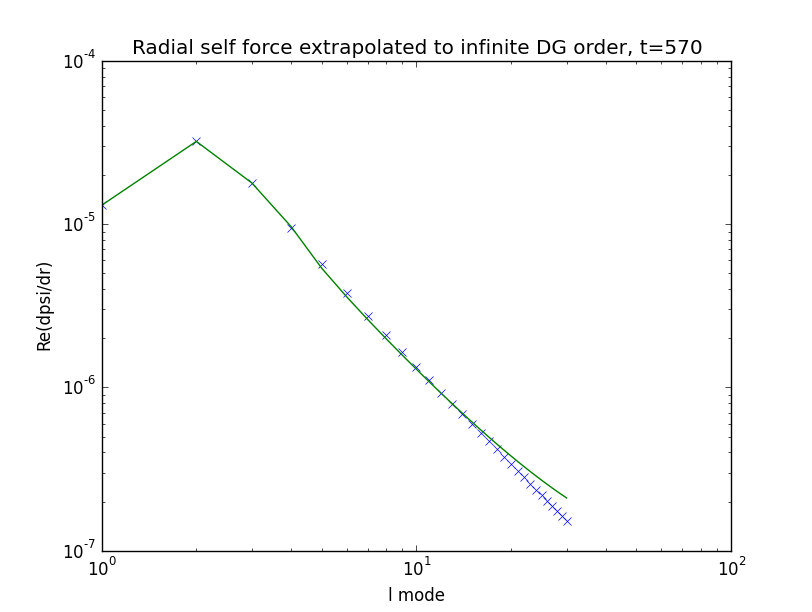
\includegraphics{finffit570}
  \caption{Three term fit of l-mode vs $F_{\inf}$.} 
\label{lmodefit}
\end{figure}

The quality of the fit depends on the number of terms in the l-mode sum used in the fit, as well as the starting and ending modes chosen. In Figure~\ref{surface234big} roundoff noise is evident at higher $l_{max}$ choices, where $l_{min}$ is the minimum l-mode included in the fit and $l_{max}$ is the maximum l-mode included in the fit. This is true of most times near aphelion. Note that there is not a large difference between two and three terms, and that four terms is less smooth a surface, suggesting that it is more subject to round off noise. Three terms is preferred. In Figure~\ref{surface234small}, a smaller region of $l_min$ versus $l_max$ space has been chosen to form the surface plot, and the roundoff noise is excluded.

\begin{figure}
  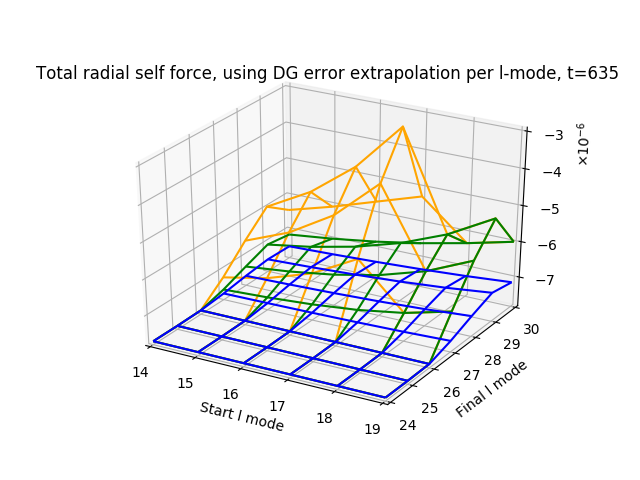
\includegraphics{bestfinflminlmax234terms635fullrange_perihelion}
  \caption{t=635, 2, 3, and 4 term fits over a broad range of lmin and lmax values. Note the roundoff noise at high lmax. Aphelion, where this effect is worst.}
  \label{surface234big}
\end{figure}

\begin{figure}
  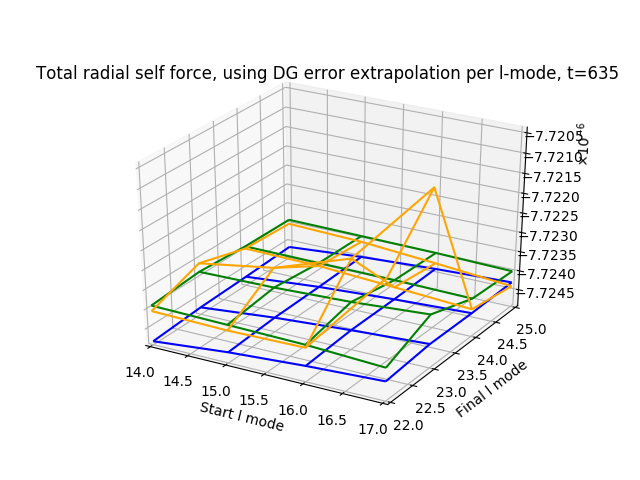
\includegraphics{bestfinflminlmax234termst635smallrange_perihelion}
  \caption{t=635, 2, 3, and 4 term fits over a small range of $l_{min}$ and $l_{max}$. Aphelion. No roundoff noise in this range.}
  \label{surface234small}
\end{figure}



Figure~\ref{totalselfforcevt} shows the evolution of the total self force over time. First it has been extrapolated to obtain $F_\infty$ using the three-point DG order exponential convergence extrapolation techique, and the optimal starting order has been chosen. Then the modes computed in the simulation have been summed numerically from $l=0$ up to some $l_{max}$, and a fit from $l_{min}$ to $l_{max}$ has been used to extrapolate the sum to infinite $l$, to obtain the total radial self-force, at each time. The three different measurement techniques described 


\begin{figure}
  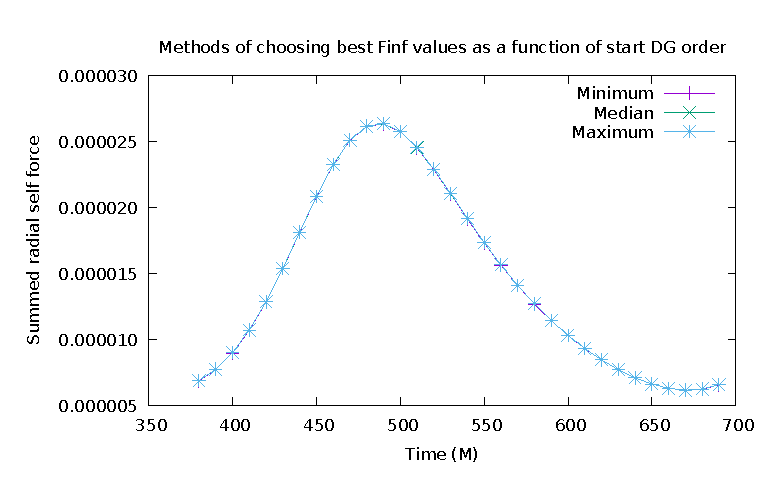
\includegraphics{bestfinfscriptplot.eps}
  \caption{This is the actual summed, doubly extrapolated, radial self force, measured using the minimum, maximum, and median method for selecting the best starting order.}
\label{totalselfforcevt}
\end{figure}



Figure~\ref{relErrSelfForceBigSmall} shows the relative difference between the total radial self force measured in two different ways. The self-force values in each surface plot shown in Figures~\ref{surface234big} and~\ref{surface234small} were averaged to obtain better estimates of the total radial self force as a function of time. This plot shows the relative difference. Some caution is advised in interpretation, since the relative difference may largely point to roundoff noise in the larger range. It is clearly random, and clearly decreasing with time, but also very clearly not at the machine precision level necessary to be roundoff noise.

\begin{figure}
  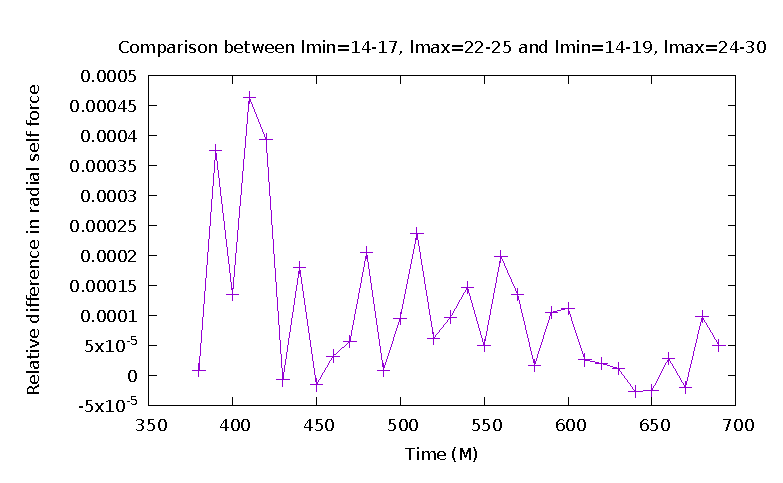
\includegraphics{relErrBigSmallRangeOverTime.eps}
  \caption{The relative difference between total self force determined by averaging large versus small ranges of total radial self-force $l_{min},l_{max}$ surfaces, as a function of time.}
  \label{relErrSelfForceBigSmall}
\end{figure}


Figure~\ref{relErr23terms} shows the relative difference between using two and three terms in the fit to compute the total radial self force, as a function of time. Again, this is random, decreasing with time, and not at the machine precision level. 


\begin{figure}
  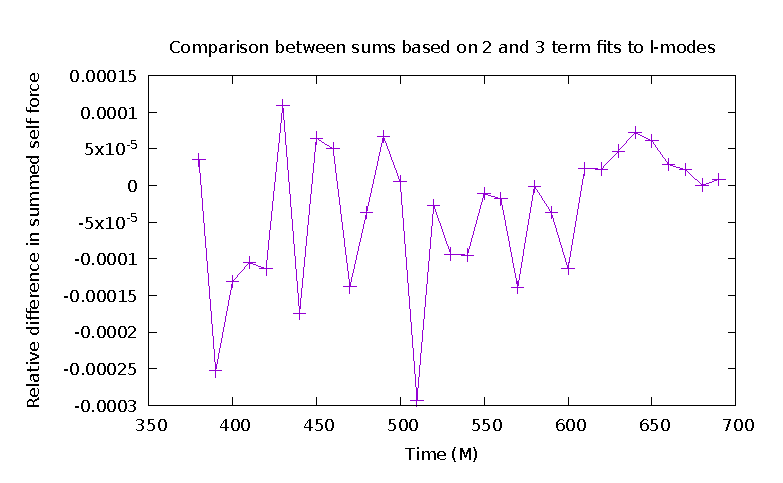
\includegraphics{relativeError23termSelfForce.eps}
  \caption{The relative error of the total radial self-force, comparing two to three terms in the l-mode fit.}
  \label{relErr23terms}
\end{figure}

In Figure~\ref{minmaxmedRelErr}, the purple line is the relative difference between the maximum and the median, and the green line is the relative difference between the median and the minimum. The first is subject to roundoff error due to the potential for the DG order with the maximum self-force, which is likely the maximum DG order, to contian roundoff error. The second is subject to effects due to failure to hit the regime where the truncation error model is valid, because of the minimum. 

\begin{figure}
  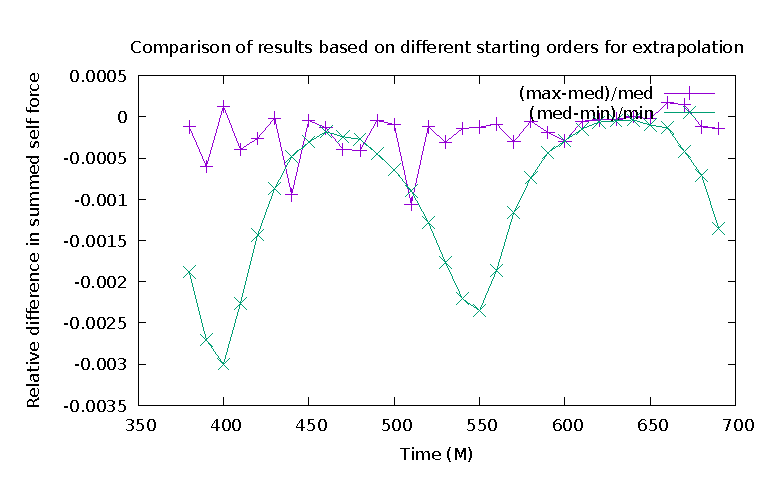
\includegraphics{minmaxmedrelativeerror3termavgl.eps}
  \caption{The relative error between median, the maximum, minimum methods of determining the starting order, summed over l-mode to obtain the total self-force and evolved over time.}
    \label{minmaxmedRelErr}
\end{figure}
  




\subsection{Fractional errors}


I obtain the fractional error, within a given method for choosing the best self force, by dividing the standard deviation of the total self-force, over a range of $l_{min}$ and $l_{max}$ by the average. This is shown for median and fit methods in Figures~\ref{medfracerr} and~\ref{fitfracerr}, respectively. The absolute error is the standard deviation itself. The absolute error, as a function of time, compared to the self-force itself, is shown in Figure~\ref{twopeaks}. The two peaks do not obviously match perihelion, aphelion, or any specific phase of the orbit. 


\begin{figure}
  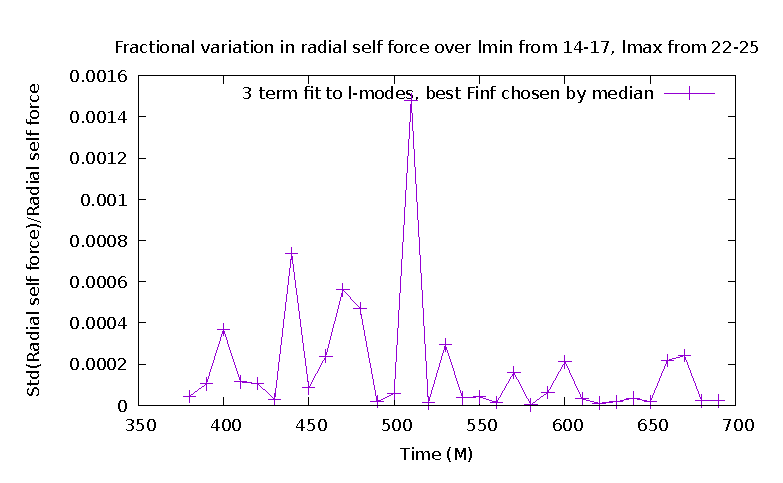
\includegraphics{fractionalErrorSelfForceOverTime3termMedian}
  \caption{Fractional error, 3 term, median method.}
  \label{medfracerr}
\end{figure}

\begin{figure}
  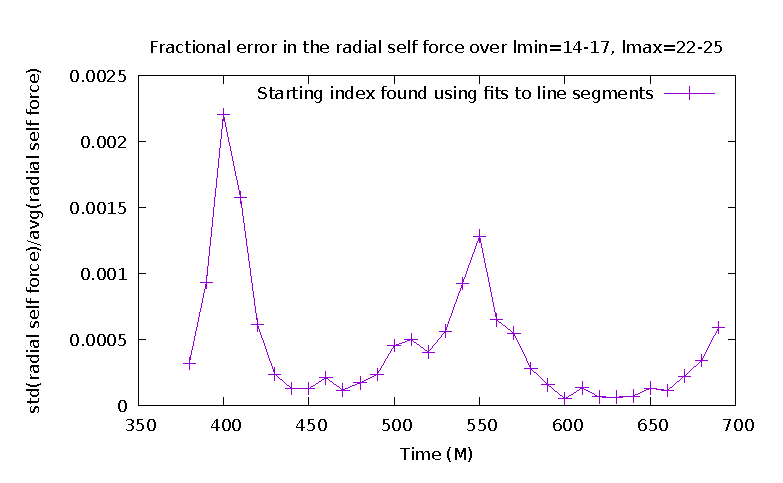
\includegraphics{fractionalErrorOverTimeFits}
  \caption{Fractional error, 3 term, fit method}
  \label{fitfracerr}
\end{figure}


\begin{figure}
  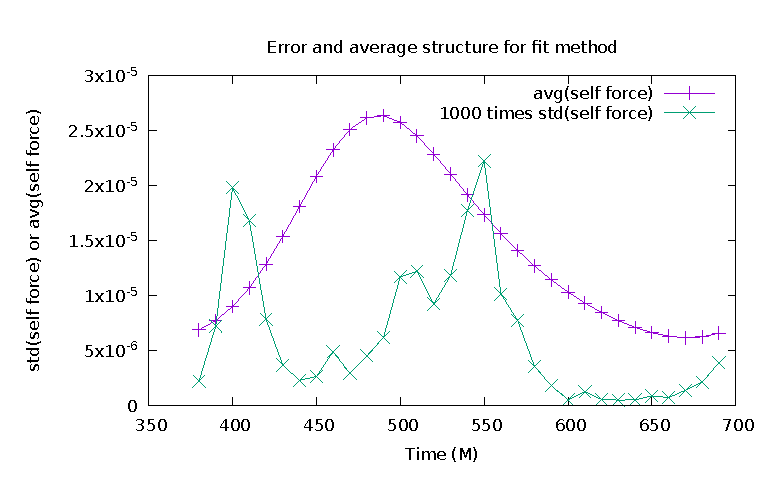
\includegraphics{structErrFitMethod}
  \caption{The structure of the absolute error in comparison to the evolution in time for the fit method.}
  \label{twopeaks}
\end{figure}





